\documentclass{article}
\usepackage{textcomp}
\usepackage{graphicx}
\usepackage{xcolor}
\usepackage[normalem]{ulem}

\definecolor{lightg}{HTML}{999999}
\definecolor{medg}{HTML}{666666}
\definecolor{darkg}{HTML}{333333}

\usepackage{wrapfig}
%FONTS
\usepackage{fontspec}
\defaultfontfeatures{Ligatures=TeX}

\font\head="Qlassik Medium:letterspace=4" at 34pt % http://www.dafont.com/qlassik.font
\font\headtwo="Qlassik Medium:letterspace=4" at 24pt % http://www.dafont.com/qlassik.font
\font\subhead="Lucida Sans Demibold Roman:mapping=tex-text" at 13pt
\font\subsubhead="Gentium Book Basic:mapping=tex-text" at 13pt
\font\subsubsubhead="Gentium Book Basic:mapping=tex-text" at 11pt
\font\Quote="Linux Libertine O Bold Italic:mapping=tex-text" at 16pt
\font\Contact="Linux Libertine O" at 9pt
\newfontfamily\Text{Linux Libertine O}[
        BoldFont={Linux Libertine O Semibold},
        ItalicFont={Linux Libertine O Italic}]

\font\Textit="Linux Libertine O/I:+onum" at 10pt
\font\HighlightFont="Linux Libertine O/I:+onum" at 10pt
\font\CvItem="Lucida Sans Regular:mapping=tex-text" at 9pt
\font\Date="Lucida Sans Demibold Roman:mapping=tex-text" at 9pt
\setmainfont[
    BoldFont={Linux Libertine O Bold},
    ItalicFont={Linux Libertine O Italic},
    BoldItalicFont={Linux Libertine O Bold Italic},
]{Linux Libertine O:mapping=tex-text}

\renewcommand\section[1]{%
    \par\vspace{1.4em}\penalty-100%
    {\subhead #1}%
    \par\penalty100\vspace{0.1em}\penalty100%
}
\renewcommand\subsection[1]{%
    \par\vspace{.1em}%
    {\hspace{0em}\subsubhead #1}%
    \par\vspace{.4em}%
}
\renewcommand\subsubsection[1]{%
    \par\vspace{.1em}%
    {\hspace{1em}\subsubsubhead #1}%
    \par\vspace{.2em}%
}
\newcommand\cvitem[2][\relax]{%
    \par\vspace{.4em}
    \if\relax#1\else{\Date \textcolor{medg}{#1}}\hspace{1em}\fi%
    {\CvItem #2}%
    \par%
}
\newcommand\showdoi[1]{%
    \href{http://dx.doi.org/#1}{[DOI]}%
}
\newcommand\preprint[1]{%
    \href{#1}{[Preprint]}%
}
\newcommand\ignore[1]{\relax}
\newcommand\pubname[1]{\textsc{\uline{#1}}}
%\newcommand\contribution[1]{\relax\hfill\break\textbf{My contribution}: \textit{#1}}
\newcommand\contribution[1]{\relax}

\newcommand\costar{${}^{*}$}
\newcommand\cosenior{†}

\usepackage[margin=1in]{geometry}
\usepackage[xetex,bookmarks,colorlinks,breaklinks]{hyperref}

\usepackage{enumitem}
\renewcommand{\labelitemi}{\textcolor{lightg}{\symbol{"F6B9}}}
\pagestyle{empty}
\begin{document}

\parindent=0cm

\begin{minipage}[t]{0.56\linewidth}%
\head LUIS PEDRO COELHO\\
\headtwo \textcolor{darkg}{Curriculum Vitæ}\\
\CvItem Sept 21, 2023 % DATE

\end{minipage}
\hfill
\begin{minipage}[t]{0.40\textwidth}%
\vspace{-2.2em}
{\Contact%
\textcolor{medg}{%
Centre for Microbiome Research\\
Queensland University of Technology\\
Brisbane, Australia}\\
\textcolor{darkg}{email} : luis@luispedro.org\\
\textcolor{darkg}{ORCID} : \href{http://orcid.org/0000-0002-9280-7885}{0000-0002-9280-7885}\\
\textcolor{darkg}{Erdös-Bacon Nr.} : 7

\textcolor{darkg}{Citizenship} : U.K.\ and Portugal
}
\end{minipage}

\section{Education}
\Text

\cvitem[2011]{PhD in computational biology, Carnegie Mellon University}
Dissertation topic: \emph{Modeling the Space of Subcellular Location Patterns
Using Images and Other Sources of Information}, advised by Prof.\ Robert F.
Murphy.

\cvitem[2006]{MSc in computer science, Instituto Superior Técnico (Technical University Lisbon)}
Dissertation topic: \emph{Bayesian Network Parameter Estimation Using Noisy
Observations or Soft Evidence}, advised by Prof.\ Arlindo Oliveira.

\cvitem[2004]{BSc in computer science, Instituto Superior Técnico (Technical University Lisbon)}
Graduated top of my class.

\section{Professional experience}

\cvitem[2023--present]{Group Leader (Queensland University of Technology)}

\cvitem[2018--2023]{Junior Principal Investigator (Fudan University)}

\cvitem[2013--2018]{Postdoctoral researcher at European Molecular Biology Laboratory (EMBL), Bork Lab}

\cvitem[2012]{Postdoctoral researcher at Instituto de Medicina Molecular (Lisbon), Mhlanga Lab}

\section{Scholarships \&\ awards}
\cvitem[2023]{ARC Future Fellowship}
\cvitem[2022]{Highly Cited Researcher (\emph{Cross-field} category)}
\cvitem[2021]{Zhicheng Teaching Award (first prize)}
\cvitem[2012]{Siebel Scholar}
Awarded annually for academic excellence and demonstrated leadership to 85 top
students from the world's leading graduate schools
\cvitem[2009]{Joint CMU-U. of Pittsburgh PhD.\ in Computational Biology Research Excellence Award}
\cvitem[2008]{Joint CMU-U. of Pittsburgh PhD.\ in Computational Biology Academic Excellence Award}
\cvitem[2006]{Fulbright Fellow}
\cvitem[2005]{Scholarship from Portuguese Science Foundation}
\cvitem[2001]{Instituto Superior Técnico (IST) Academic Excellence Award}

\section{Highlighted publications}
\cvitem[2022]{\HighlightFont \textbf{L. P. Coelho} et al. \emph{Towards the biogeography of
prokaryotic genes} in \pubname{Nature} \showdoi{10.1038/s41586-021-04233-4}}
\cvitem[2022]{\HighlightFont S. Pan, \ldots, \textbf{L. P. Coelho} \emph{A deep
siamese neural network improves metagenome-assembled genomes in microbiome
datasets across different environments} in \pubname{Nature Communications}
\showdoi{10.1038/s41467-022-29843-y}}
\cvitem[2018]{\HighlightFont \textbf{L. P. Coelho} et al., \emph{Similarity of the dog and
human gut microbiomes in gene content and response to diet} in
\pubname{Microbiome} \showdoi{10.1186/s40168-018-0450-3}}
\cvitem[2015]{\HighlightFont S. Sunagawa\costar, \textbf{L. P. Coelho}\costar, S.
    Chaffron\costar et al., \emph{Structure and Function of the Global Ocean
Microbiome} in \pubname{Science} \showdoi{10.1126/science.1261359}}
\break
\section{Grants awarded (selected)}
\cvitem[2022]{Studying small proteins of the global microbiome using deep learning, Shanghai Municipal Science and Technology Commission (SMSTC)}
\cvitem[2020]{Establishing a Monitoring Baseline for Antibiotic Resistance in Key environments (EMBARK)}
International consortium to work on antimicrobial resistance, funded through JPI-AMR.
\cvitem[2019]{Using deep learning to understand the microbiome, National Science Foundation of China}

\section{Service \& outreach (selected)}
\cvitem[2021--present]{Member of the steering committee for mVIF (Microbiome Virtual International Forum)}
\cvitem[2021--2023]{Academic Editor for PLoS Computational Biology}
\cvitem[2020--present]{Member of the ISCB (International Society for
Computational Biology) Equity, Diversity and Inclusion (EDI) Committee}
\cvitem[2016--2021]{Associate Editor for the Journal of Open Research Software}
\cvitem[2014--2017]{Postdoc representative at EMBL}
I helped organized the 2015 and 2017 EMBL Postdoc retreats.
\cvitem[2014--2015]{Organized Software Carpentry Workshop at EMBL}
\cvitem[2012--2013]{Member of the Organization of the Lisbon Machine Learning School}
\cvitem[2010]{Local Committee for Portuguese-American Postgraduate Society National Forum}

\section{Teaching \& mentoring (selected)}
\cvitem[2019--2023]{Co-taught \emph{Scientific Communication} at Fudan University, a one-semester graduate course}
\cvitem[2012--present]{Certified Software Carpentry Instructor}
I have given lectures on Software Carpentry in Germany, Denmark, Cyprus, Jordan, and Spain.
\cvitem[2009]{Programming for Scientists}
I designed and taught a semester-long course on computer programming for
scientists at Carnegie Mellon University.
\cvitem[2008]{Teaching Assistant for Laboratory Methods for Computational Biologists (CMU)}

\section{Bibliometric statistics}

\textbf{Total number of citations}: 14,436 (Google Scholar); 9,276 (Web of Science)
\\
\textbf{h-index}: 41 (Google Scholar); 34 (Web of Science)

\begin{center}
    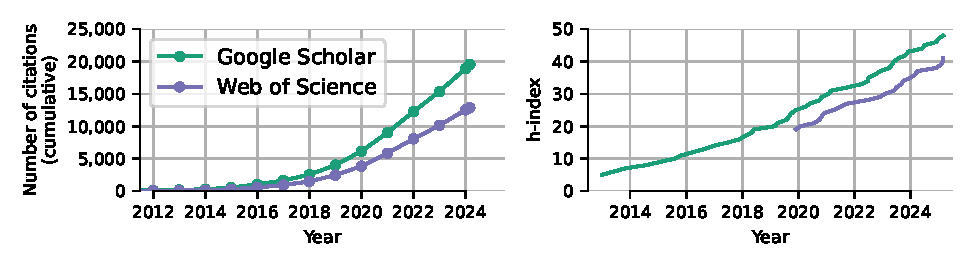
\includegraphics{citations-h-index.pdf}
\end{center}

\section{Language skills}

Native speaker of \textbf{English} and \textbf{Portuguese}; fluent in
\textbf{German} and \textbf{French}; basic \textbf{Luxembourgish}.


\pagebreak
\section{Publications}

Google scholar profile: \\
\href%
    {http://scholar.google.com/citations?user=qTYua0cAAAAJ}%
    {http://scholar.google.com/citations?user=qTYua0cAAAAJ}

\medskip

\medskip


\section{First or corresponding author}
{\small (includes co-first/co-corresponding author publications)}
\vspace{2em}

\subsubsection{Preprints submitted for publication}

\begin{enumerate}

\item Célio Dias Santos-Júnior\costar, Marcelo Der Torossian Torres\costar, Yiqian Duan, Álvaro Rodríguez del Río, Thomas S.B. Schmidt, Hui Chong, Anthony Fullam, Kuhn Michael, Chengkai Zhu, Amy Houseman, Jelena Somborski, Anna Vines, Xing-Ming Zhao, Peer Bork, Jaime Huerta-Cepas, Cesar de la Fuente-Nunez⁺, \textbf{Luis Pedro Coelho}⁺ \emph{Computational exploration of the global microbiome for antibiotic discovery} in \pubname{bioRxiv (PREPRINT)} 2023 \showdoi{10.1101/2023.08.31.555663}

\item Marija Dmitrijeva, Janko Tackmann, João Matias Rodrigues, Jaime Huerta-Cepas, \textbf{Luis Pedro Coelho}⁺, Christian von Mering⁺ \emph{A global survey of eco-evolutionary pressures acting on horizontal gene transfer} in \pubname{Research Square (PREPRINT)} 2023 \showdoi{10.21203/rs.3.rs-3062985/v1}

\end{enumerate}

\subsubsection{Peer-reviewed journal publications}

\begin{enumerate}[resume]

\item Shaojun Pan, Xing-Ming Zhao⁺, \textbf{Luis Pedro Coelho}⁺, \emph{SemiBin2: self-supervised contrastive learning leads to better MAGs for short- and long-read sequencing} in \pubname{Bioinformatics} (Accepted) 2023 \showdoi{10.1101/2023.01.09.523201} (preprint)

\item Senying Lai, Shaojun Pan, \textbf{Luis Pedro Coelho}⁺, Wei-Hua Chen,⁺
Xing-Ming Zhao⁺, \emph{metaMIC: reference-free Misassembly Identification and
Correction of de novo metagenomic assemblies} in \pubname{Genome Biology} 2022
\showdoi{10.1186/s13059-022-02810-y}


\item Shaojun Pan, Chengkai Zhu, Xing-Ming Zhao⁺, and \textbf{Luis Pedro
Coelho}⁺ \emph{A deep siamese neural network improves metagenome-assembled
genomes in microbiome datasets across different environments} in
\pubname{Nature Communications} 2022 \showdoi{10.1038/s41467-022-29843-y}

\item \textbf{Luis Pedro Coelho}, Renato Alves, Álvaro Rodríguez del Río,
Pernille Neve Myers, Carlos P. Cantalapiedra, Joaquín Giner-Lamia,Thomas
Sebastian Schmidt, Daniel R. Mende, Askarbek Orakov, Ivica Letunic, Falk
Hildebrand, Thea Van Rossum, Sofia K. Forslund, Supriya Khedkar, Oleksandr M.
Maistrenko, Shaojun Pan, Longhao Jia, Pamela Ferretti, Shinichi Sunagawa,
Xing-Ming Zhao, Henrik Bjørn Nielsen, Jaime Huerta-Cepas⁺, and Peer Bork⁺,
\emph{Towards the biogeography of prokaryotic genes} in \pubname{Nature} 2022
\showdoi{10.1038/s41586-021-04233-4}

\item Célio Dias Santos-Junior, Shaojun Pan, Xing-Ming Zhao, \textbf{Luis Pedro
Coelho}, \emph{MACREL: antimicrobial peptide screening in genomes and
metagenomes} in \pubname{PeerJ} 2020 \showdoi{10.7717/peerj.10555}

\item \textbf{Luis Pedro Coelho}, Renato Alves, Paulo Monteiro, Jaime
Huerta-Cepas, Ana Teresa Freitas, Peer Bork \emph{NG-meta-profiler: fast
processing of metagenomes using NGLess, a domain-specific language} in
\pubname{Microbiome} vol.\ 7, 84, 2019 \showdoi{10.1186/s40168-019-0684-8}
\contribution{I conceived of the concept, co-wrote the software and the manuscript}

\item \textbf{Luis Pedro Coelho}, Jens Kultima, Paul Costea, Coralie Fournier,
Yuanlong Pan, Gail Czarnecki-Maulden, Matthew Hayward, Kristoffer Forslund,
Patrick Descombes, Janet Jackson, Qinghong Li, and Peer Bork \emph{Similarity
of the dog and human gut microbiomes in gene content and response to diet} in
\pubname{Microbiome}, vol 6:72, 2018 \showdoi{10.1186/s40168-018-0450-3}
\contribution{I designed and implemented the analysis strategy, wrote the first
version of the manuscript, and lead the subsequent incorporation of co-author
suggestions.}

\item \textbf{Luis Pedro Coelho}, \emph{Jug: Software for parallel reproducible
computation in Python} in \pubname{Journal of Open Research
Software}, 2017 \showdoi{10.5334/jors.161}
\contribution{I designed and implemented the software presented and wrote the
manuscript.}

\item Sebastien Colin\costar, \textbf{Luis Pedro Coelho}\costar, Shinichi
Sunagawa, Chris Bowler, Eric Karsenti, Peer Bork, Rainer Pepperkok, Colomban de
Vargas, \emph{Quantitative 3D-imaging for cell biology and ecology of
environmental microbial eukaryotes} in \pubname{eLife}, vol.\ 6:e26066, 2017
\showdoi{10.7554/eLife.26066.001}
\contribution{I designed and implemented the computational analysis necessary
for the method presented in the paper and participated in the writing of the
manuscript.}

\item Shinichi Sunagawa\costar, \textbf{Luis Pedro Coelho}\costar, Samuel
Chaffron\costar, Jens Roat Kultima, Karine Labadie, Guillem Salazar, Bardya
Djahanschiri, Georg Zeller, Daniel R. Mende, Adriana Alberti, Francisco M.
Cornejo-Castillo, Paul I. Costea, Corinne Cruaud, Francesco d'Ovidio, Stefan
Engelen, Isabel Ferrera, Josep M. Gasol, Lionel Guidi, Falk Hildebrand, Florian
Kokoszka, Cyrille Lepoivre, Gipsi Lima-Mendez, Julie Poulain, Bonnie T. Poulos,
Marta Royo-Llonch, Hugo Sarmento, Sara Vieira-Silva, Céline Dimier, Marc
Picheral, Sarah Searson, Stefanie Kandels-Lewis, Tara Oceans coordinators,
Chris Bowler, Colomban de Vargas, Gabriel Gorsky, Nigel Grimsley, Pascal
Hingamp, Daniele Iudicone, Olivier Jaillon, Fabrice Not, Hiroyuki Ogata,
Stephane Pesant, Sabrina Speich, Lars Stemmann, Matthew B. Sullivan, Jean
Weissenbach, Patrick Wincker, Eric Karsenti, Jeroen Raes, Silvia G. Acinas,
Peer Bork, \emph{Structure and Function of the Global Ocean Microbiome} in
\pubname{Science} 348 (6237), 1261359, 2015 \showdoi{10.1126/science.1261359}
\contribution{As co-first author, I performed analysis of the data, including
linking the metagenomics data to the environmental parameters, as well as the
comparison to the human gut (this required extending existing software tools
which were unable to scale to this dataset); and helped draft the manuscript.}

\item \textbf{Luis Pedro Coelho}, Catarina Pato, Ana Friães, Ariane Neumann,
Maren von Köckritz-Blickwede, Mário Ramirez, João André Carriço,
\emph{Automatic determination of NET (neutrophil extracellular traps) coverage
in fluorescent microscopy images} in \pubname{Bioinformatics} 31 (14):
2364--2370, 2015 \showdoi{10.1093/bioinformatics/btv156}
\contribution{I conceived and implemented the algorithm, and wrote the
manuscript.}

\item \textbf{Luis Pedro Coelho}, Joshua D. Kangas, Armaghan Naik, Elvira
Osuna-Highley, Estelle Glory-Afshar, Margaret Fuhrman, Ramanuja Simha, Peter B.
Berget, Jonathan W. Jarvik, and Robert F. Murphy, \emph{Determining the
subcellular location of new proteins from microscope images using local
features} in \pubname{Bioinformatics}, 2013 \showdoi{10.1093/bioinformatics/btt392}
\contribution{I designed and implemented the proposed algorithm, collected
microscopy data (in collaboration with other authors), and wrote the
manuscript.}

\item \textbf{Luis Pedro Coelho} \emph{Mahotas: Open source software for
scriptable computer vision}, \pubname{Journal of Open Research Software}, vol.\
1, 2013 \showdoi{10.5334/jors.ac}
\contribution{I implemented the underlying computer vision software and the manuscript.}

\item \textbf{Luis Pedro Coelho}\costar, Tao Peng\costar, and Robert F.
Murphy, \emph{Quantifying the distribution of probes between subcellular
locations using unsupervised pattern unmixing} in \pubname{Bioinformatics},
vol.\ 26 (12), pp.\ i7--i12, 2010 \showdoi{10.1093/bioinformatics/btq220}
\contribution{I conceived of and implemented one of the methods presented and
wrote the manuscript.}

\item \textbf{Luis Pedro Coelho}, Amr Ahmed, Andrew Arnold, Joshua Kangas,
Abdul-Saboor Sheikh, Eric P. Xing, William W. Cohen, and Robert F. Murphy,
\emph{Structured Literature Image Finder: Extracting Information from Text and
Images in Biomedical Literature} in \pubname{Lecture Notes in Bioinformatics},
vol.\ 6004, pp.\ 23--32, 2010 \showdoi{10.1007/978-3-642-13131-8_4}
\contribution{With the paper below, this forms a package on the SLIF project,
where I enhanced the image analysis pipeline (for the analysis of figures in
published scientific literature). I wrote the first draft of this manuscript
and helped draft the one below.}

\end{enumerate}

\subsubsection{Peer-reviewed Conference Proceedings}

\begin{enumerate}[resume]
\item \textbf{Luis Pedro Coelho}, Aabid Shariff, and Robert F. Murphy;
\emph{Nuclear segmentation in microscope cell images: A hand-segmented dataset
and comparison of algorithms} in \pubname{Proceedings of IEEE International
Symposium in Biomedical Imaging}, 2009 \showdoi{10.1109/ISBI.2009.5193098}
\contribution{I acquired (part of) the microscopy data, built the
hand-segmented dataset, implemented the methods and wrote the first draft of
the manuscript.}


\item \textbf{Luis Pedro Coelho} and Robert Murphy; \emph{Identifying
Subcellular Locations from Images of Unknown Resolution} in
\pubname{Bioinformatics Research and Development}, Communications in Computer
and Information Science, vol.\ 13, pp.\ 235--242, 2008
\showdoi{10.1007/978-3-540-70600-7_18}
\contribution{I implemented the algorithm, ran the tests, and wrote the first
draft of the paper.}

\item \textbf{Luis Pedro Coelho} and Arlindo Oliveira; \emph{Dotted Suffix
Trees: A Structure for Approximate Text Indexing} in \pubname{String Processing
and Information Retrieval}, Lecture Notes in Computer Science, vol.\ 4209, pp.\
329--336, 2006 \showdoi{10.1007/11880561_27}
\contribution{I developed and implemented the algorithm and wrote the first
draft of the manuscript.}

\end{enumerate}

\subsubsection{Comments and review articles}

\begin{enumerate}[resume]

\item \textbf{Luis Pedro Coelho} \emph{Voices of the new generation: science in
a state of benign confusion} in \pubname{Nature Reviews Molecular Cell Biology}
2020 \showdoi{10.1038/s41580-020-0265-5}

\item \textbf{Luis Pedro Coelho}, Estelle Glory-Afshar, Joshua Kangas, Shannon
Quinn, Aabid Shariff, and Robert F. Murphy; \emph{Principles of Bioimage
Informatics: Focus on machine learning of cell patterns} in \pubname{Linking
Literature, Information, and Knowledge for Biology}, Lecture Notes in Computer
Science, vol.  6004, pp. 8--18, 2010 \showdoi{10.1007/978-3-642-13131-8_2}

\end{enumerate}

\break
\section{Co-authorships}

\subsubsection{Preprints submitted for publication}

\begin{enumerate}[resume]

\item Álvaro Rodríguez del Río, Joaquín Giner-Lamia, Carlos P. Cantalapiedra, Jorge Botas, Ziqi Deng, Ana Hernández-Plaza, Lucas Paoli, Thomas S.B. Schmidt, Shinichi Sunagawa, Peer Bork,  \textbf{Luis Pedro Coelho}, Jaime Huerta-Cepas \emph{Functional and evolutionary significance of unknown genes from uncultivated taxa} in \pubname{BioRxiv} 2022 \showdoi{10.1101/2022.01.26.477801}

\end{enumerate}

\subsubsection{Peer-reviewed journal publications}

\begin{enumerate}[resume]

\item Johan Bengtsson-Palme, Anna Abramova, Thomas U. Berendonk, \textbf{Luis Pedro Coelho}, Sofia K. Forslund, Rémi Gschwind, Annamari Heikinheimo, Víctor Hugo Jarquín-Díaz, Ayaz Ali Khan, Uli Klümper, Ulrike Löber, Marmar Nekoro, Adriana D. Osińska, Svetlana Ugarcina Perovic, Tarja Pitkänen, Ernst Kristian Rødland, Etienne Ruppé, Yngvild Wasteson, Astrid Louise Wester, Rabaab Zahra \emph{Towards Monitoring of Antimicrobial Resistance in the Environment: For what Reasons, How to Implement It, and What Are the Data Needs?} in \pubname{Environment International} 2023 \showdoi{10.1016/j.envint.2023.108089}

\item Rémi Gschwind, Svetlana Ugarcina Perovic, Marie Petitjean, Julie Lao, \textbf{Luis Pedro Coelho}, Etienne Ruppé \emph{ResFinderFG v2.0: a database of antibiotic resistance genes obtained by functional metagenomics} in \pubname{Nucleic Acid Research} 2023 \showdoi{10.1093/nar/gkad384}

\item Hui Chong, Qingyang Yu, Yuguo Zha, Guangzhou Xiong, Nan Wang, Xinhe Huang, Shijuan Huang, Chuqing Sun, Sicheng Wu, Wei-Hua Chen, \textbf{Luis Pedro Coelho}, Kang Ning \emph{EXPERT: Transfer Learning-enabled context-aware microbial source tracking} in \pubname{Briefings in Bioinformatics} 2022 \showdoi{10.1093/bib/bbac396}

\item Thomas SB Schmidt, Simone S Li, Oleksandr M Maistrenko, Wasiu Akkani, \textbf{Luis Pedro Coelho}, Sibasish Dolai, Anthony Fullam, Anna Glazek, Rajna Hercog, Hilde Herrema, Ferris Jung, Stefanie Kandels, Askarbek Orakov, Thea Van Rossum, Vladimir Benes, Thomas J Borody, Willem M de Vos, Cyriel Y Ponsioen, Max Nieuwdorp, Peer Bork \emph{Drivers and Determinants of Strain Dynamics Following Faecal Microbiota Transplantation} in \pubname{Nature Medicine} 2022 \showdoi{10.1038/s41591-022-01913-0}

\item Sebastien Fromentin, Sofia K. Forslund, Kanta Chechi, Judith Aron-Wisnewsky, Rima Chakaroun, Trine Nielsen, Valentina Tremaroli, Boyang Ji, Edi Prifti, Antonis Myridakis, Julien Chilloux, Petros Andrikopoulos, Yong Fan, Michael T. Olanipekun, Renato Alves, Solia Adiouch, Noam Bar, Yeela Talmor-Barkan, Eugeni Belda, Robert Caesar, \textbf{Luis Pedro Coelho}, Gwen Falony, Soraya Fellahi, Pilar Galan, Nathalie Galleron, Gerard Helft, Lesley Hoyles, Richard Isnard, Emmanuelle Le Chatelier, Hanna Julienne, Lisa Olsson, Helle Krogh Pedersen, Nicolas Pons, Benoit Quinquis, Christine Rouault, Hugo Roume, Joe-Elie Salem, Thomas S. B. Schmidt, Sara Vieira-Silva, Peishun Li, Maria Zimmermann-Kogadeeva, Christian Lewinter, Nadja B. Søndertoft, Tue H. Hansen, Dominique Gauguier, Jens Peter Gøtze, Lars Køber, Ran Kornowski, Henrik Vestergaard, Torben Hansen, Jean-Daniel Zucker, Serge Hercberg, Ivica Letunic, Fredrik Bäckhed, Jean-Michel Oppert, Jens Nielsen, Jeroen Raes, Peer Bork, Michael Stumvoll, Eran Segal, Karine Clément\cosenior, Marc-Emmanuel Dumas\cosenior, S. Dusko Ehrlich\cosenior, and Oluf Pedersen\cosenior \emph{Microbiome and metabolome features of the cardiometabolic disease spectrum} at \pubname{Nature Medicine} 2022 \showdoi{10.1038/s41591-022-01688-4}

\item Supriya Khedkar, Georgy Smyshlyaev, Ivica Letunic, Oleksandr M Maistrenko, \textbf{Luis Pedro Coelho}, Askarbek Orakov, Sofia K Forslund, Falk Hildebrand, Mechthild Luetge, Thomas S B Schmidt, Orsolya Barabas, and Peer Bork \emph{Landscape of mobile genetic elements and their antibiotic resistance cargo in prokaryotic genomes} in \pubname{Nucleic Acids Research} 2022 \showdoi{10.1093/nar/gkac163}

\item Eugeni Belda\costar, Lise Voland\costar, Valentina Tremaroli\costar, Gwen Falony\costar, Solia Adriouch\costar, Karen E Assmann\costar, Edi Prifti, Judith Aron-Wisnewsky, Jean Debédat, Tiphaine Le Roy, Trine Nielsen, Chloé Amouyal, Sébastien André, Fabrizio Andreelli, Matthias Blüher, Rima Chakaroun, Julien Chilloux, \textbf{Luis Pedro Coelho}, Maria Carlota Dao, Promi Das, Soraya Fellahi, Sofia Forslund, Nathalie Galleron, Tue H Hansen, Bridget Holmes, Boyang Ji, Helle Krogh Pedersen, Phuong Le, Emmanuelle Le Chatelier, Christian Lewinter, Louise Mannerås-Holm, Florian Marquet, Antonis Myridakis, Veronique Pelloux, Nicolas Pons, Benoit Quinquis, Christine Rouault, Hugo Roume, Joe-Elie Salem, Nataliya Sokolovska, Nadja B Søndertoft, Sothea Touch, Sara Vieira-Silva, The MetaCardis Consortium, Pilar Galan, Jens Holst, Jens Peter Gøtze, Lars Køber, Henrik Vestergaard, Torben Hansen, Serge Hercberg, Jean-Michel Oppert, Jens Nielsen, Ivica Letunic, Marc-Emmanuel Dumas, Michael Stumvoll, Oluf Borbye Pedersen, Peer Bork, Stanislav Dusko Ehrlich, Jean-Daniel Zucker, Fredrik Bäckhed, Jeroen Raes, and Karine Clément \emph{Impairment of gut microbial biotin metabolism and host biotin status in severe obesity: effect of biotin and prebiotic supplementation on improved metabolism} at \pubname{Gut} 2022 \showdoi{10.1136/gutjnl-2021-325753}

\item Boas C.L. van der Putten\costar, C. I. Mendes\costar, Brooke M. Talbot, Jolinda de Korne-Elenbaas, Rafael Mamede, Pedro Vila-Cerqueira, \textbf{Luis Pedro Coelho},  Christopher A. Gulvik, Lee S. Katz, and The ASM NGS 2020 Hackathon participants \emph{Software testing in microbial bioinformatics: a call to action} at \pubname{Microbial Genomics} 2022 \showdoi{10.1099/mgen.0.000790}

\item Sofia K. Forslund\costar, Rima Chakaroun\costar, Maria
Zimmermann-Kogadeeva\costar, Lajos Markó\costar, Judith Aron-Wisnewsky\costar,
Trine Nielsen\costar, Lucas Moitinho-Silva, Thomas S. B.  Schmidt, Gwen Falony,
Sara Vieira-Silva, Solia Adriouch, Renato J. Alves, Karen Assmann,
Jean-Philippe Bastard, Till Birkner, Robert Caesar, Julien Chilloux,
\textbf{Luis Pedro Coelho}, Leopold Fezeu, Nathalie Galleron, Gerard Helft,
Richard Isnard, Boyang Ji, Michael Kuhn, Emmanuelle Le Chatelier, Antonis
Myridakis, Lisa Olsson, Nicolas Pons, Edi Prifti, Benoit Quinquis, Hugo Roume,
Joe-Elie Salem, Nataliya Sokolovska, Valentina Tremaroli, Mireia
Valles-Colomer, Christian Lewinter, Nadja B Søndertoft, Helle Krogh Pedersen,
Tue H Hansen, \textit{The MetaCardis Consortium}, Jens Peter Gøtze, Lars Køber,
Henrik Vestergaard9,25, Torben Hansen9, Jean-Daniel Zucker7,20,21, Serge
Hercberg, Jean-Michel Oppert, Ivica Letunic, Jens Nielsen, Fredrik Bäckhed, S.
Dusko Ehrlich, Marc-Emmanuel Dumas, Jeroen Raes, Oluf Pedersen, Karine
Clément\cosenior, Michael Stumvoll\cosenior, Peer Bork\cosenior
\emph{Combinatorial, additive and dose-dependent drug- microbiome associations}
at \pubname{Nature} 2021 \showdoi{10.1038/s41586-021-04177-9}

\item Askarbek Orakov\costar, Anthony Fullam\costar, \textbf{Luis Pedro
Coelho}, Supriya Khedkar, Damian Szklarczyk, Daniel R Mende, Thomas SB Schmidt†
and Peer Bork† \emph{GUNC: Detection of Chimerism and Contamination in
Prokaryotic Genomes} at \pubname{Genome Biology} 2021
\showdoi{10.1186/s13059-021-02393-0}

\item Mohammad Bahram, Tarquin Netherway, Clémence Frioux, Pamela Ferretti,
\textbf{Luis Pedro Coelho}, Stefan Geisen, Peer Bork, and Falk Hildebrand
\emph{Metagenomic assessment of the global diversity and distribution of
bacteria and fungi} at \pubname{Environmental Microbiology} 2020
\showdoi{10.1111/1462-2920.15314}

\item Sara Vieira-Silva, Gwen Falony, Eugeni Belda, Trine Nielsen, Judith
Aron-Wisnewsky, Rima Chakaroun, Sofia K. Forslund, Karen Assmann, Mireia
Valles-Colomer, Thi Thuy Duyen Nguyen, Sebastian Proost, Edi Prifti, Valentina
Tremaroli, Nicolas Pons, Emmanuelle Le Chatelier, Fabrizio Andreelli,
Jean-Phillippe Bastard, \textbf{Luis Pedro Coelho}, Nathalie Galleron, Tue H.
Hansen, Jean-Sébastien Hulot, Christian Lewinter, Helle K. Pedersen, Benoit
Quinquis, Christine Rouault, Hugo Roume, Joe-Elie Salem, Nadja B. Søndertoft,
Sothea Touch, MetaCardis Consortium, Marc-Emmanuel Dumas, Stanislav Dusko
Ehrlich, Pilar Galan, Jens P. Gøtze, Torben Hansen, Jens J. Holst, Lars Køber,
Ivica Letunic, Jens Nielsen, Jean-Michel Oppert, Michael Stumvoll, Henrik
Vestergaard, Jean-Daniel Zucker, Peer Bork, Oluf Pedersen, Fredrik Bäckhed,
Karine Clément and Jeroen Raes \emph{Statin therapy is associated with lower
prevalence of gut microbiota dysbiosis} in \pubname{Nature} 581, 310–315 (2020)
\showdoi{10.1038/s41586-020-2269-x}

\item Oleksandr M. Maistrenko\costar,  Daniel R. Mende\costar,  Mechthild
Luetge, Falk Hildebrand,  Thomas S. B. Schmidt,  Simone S. Li, \textbf{Luis
Pedro Coelho},  Jaime Huerta-Cepas,  Shinichi Sunagawa,  Peer Bork
\emph{Disentangling the impact of environmental and phylogenetic constraints on
prokaryotic within-species diversity} in \pubname{ISME Journal} 14, 1247–1259
2020 \showdoi{10.1038/s41396-020-0600-z}

\item Daniel R Mende, Ivica Letunic, Oleksandr M Maistrenko, Thomas S B Schmidt,
Alessio Milanese, Lucas Paoli, Ana Hernández-Plaza, Askarbek N Orakov, Sofia K
Forslund, Shinichi Sunagawa, Georg Zeller, Jaime Huerta-Cepas, \textbf{Luis
Pedro Coelho}, Peer Bork \emph{proGenomes2: an improved database for accurate
and consistent habitat, taxonomic and functional annotations of prokaryotic
genomes} in \pubname{Nucleic Acids Research} 48:D1 D621-D625, 2020
\showdoi{10.1093/nar/gkz1002}

\item Federico M. Ibarbalz, Nicolas Henry, Manoela C. Brandão, Séverine
Martini, Greta Busseni, Hannah Byrne, \textbf{Luis Pedro Coelho}, Hisashi Endo,
Josep M. Gasol, Ann C. Gregory, Frédéric Mahé, Janaina Rigonato, Marta
Royo-Llonch, Guillem Salazar, Isabel Sanz-Sáez, Eleonora Scalco, Dodji
Soviadan, Ahmed A. Zayed, Adriana Zingone, Karine Labadie, Joannie Ferland,
Claudie Marec, Stefanie Kandels, Marc Picheral, Céline Dimier, Julie Poulain,
Sergey Pisarev, Margaux Carmichael, Stéphane Pesant, Tara Oceans Coordinators,
Marcel Babin, Emmanuel Boss, Daniele Iudicone, Olivier Jaillon, Silvia G.
Acinas, Hiroyuki Ogata, Eric Pelletier, Lars Stemmann, Matthew B. Sullivan,
Shinichi Sunagawa, Laurent Bopp, Colomban de Vargas, Lee Karp-Boss, Patrick
Wincker, Fabien Lombard, Chris Bowler\#, and Lucie Zinger\# \emph{Global Trends
in Marine Plankton Diversity across Kingdoms of Life} in \pubname{Cell}, 2019
\showdoi{10.1016/j.cell.2019.10.008}

\item Guillem Salazar\costar, Lucas Paoli\costar, Adriana Alberti, Jaime
Huerta-Cepas, Hans-Joachim Ruscheweyh, Miguelangel Cuenca, Christopher M.
Field, \textbf{Luis Pedro Coelho}, Corinne Cruaud, Stefan Engelen, Ann C.
Gregory, Karine Labadie, Claudie Marec, Eric Pelletier, Marta Royo-Llonch,
Simon Roux, Pablo Sánchez, Hideya Uehara, Ahmed A. Zayed, Georg Zeller,1Margaux
Carmichael, Céline Dimier, Joannie Ferland, Stefanie Kandels, Marc Picheral,
Sergey Pisarev, Julie Poulain, Tara Oceans Coordinators, Silvia G. Acinas,
Marcel Babin, Peer Bork, Chris Bowler, Colomban de Vargas, Lionel Guidi, Pascal
Hingamp, Daniele Iudicone, Lee Karp-Boss, Eric Karsenti, Hiroyuki Ogata,
Stephane Pesant, Sabrina Speich, Matthew B. Sullivan, Patrick Wincker, and
Shinichi Sunagawa, \emph{Gene Expression Changes and Community Turnover
Differentially Shape the Global Ocean Metatranscriptome} in \pubname{Cell},
2019 \showdoi{10.1016/j.cell.2019.10.014}

\item Jakob Wirbel\costar, Paul Theodor Pyl\costar, Ece Kartal, Konrad Zych,
Alireza Kashani, Alessio Milanese, Jonas S Fleck, Anita Y Voigt, Albert
Palleja, Ruby P Ponnudurai, Shinichi Sunagawa, \textbf{Luis Pedro Coelho},
Petra Schrotz-King, Emily Vogtmann, Nina Habermann, Emma Niméus, Andrew M
Thomas, Paolo Manghi, Sara Gandini, Davide Serrano, Sayaka Mizutani, Hirotsugu
Shiroma, Satoshi Shiba, Tatsuhiro Shibata, Shinichi Yachida, Takuji Yamada,
Levi Waldron, Alessio Naccarati, Nicola Segata, Rashmi Sinha, Cornelia M.
Ulrich, Hermann Brenner, Manimozhiyan Arumugam, Peer Bork, Georg Zeller
\emph{Meta-analysis of fecal metagenomes reveals global microbial signatures
that are specific for colorectal cancer} in \pubname{Nature Medicine} vol.\ 25,
pp.\ 679–689 (2019) \showdoi{10.1038/s41591-019-0406-6}

\item Alessio Milanese\costar, Daniel Mende\costar, Lucas Paoli, Guillem
Salazar, Hans-Joachim Ruscheweyh, Miguelangel Cuenca, Pascal Hingamp, Renato
Alves, Paul Costea, \textbf{Luis Pedro Coelho}, Thomas Schmidt, Alexandre
Almeida, Alex Mitchell, Robert Finn, Jaime Huerta-Cepas, Peer Bork, Georg
Zeller, and Shinichi Sunagawa \emph{Microbial abundance, activity and
population genomic profiling with mOTUs2} in \pubname{Nature Communications},
vol.\ 10, pp. 1014, 2019 \showdoi{10.1038/s41467-019-08844-4}

\item Thomas SB Schmidt\costar, Matthew R Hayward\costar, \textbf{Luis Pedro
Coelho}, Simone S Li, Paul I Costea, Anita Y Voigt, Jakob Wirbel, Oleksandr M
Maistrenko, Renato J Alves, Emma Bergsten, Carine de Beaufort, Iradj Sobhani,
Anna Heintz-Buschart, Shinichi Sunagawa, Georg Zeller, Paul Wilmes, Peer Bork
\emph{Extensive Transmission of Microbes along the Gastrointestinal Tract} in
\pubname{eLife}, vol.\ 8, pp.\ e42693, 2019 \showdoi{10.7554/eLife.42693}

\item Luigi Caputi\costar, Quentin Carradec\costar, Damien Eveillard\costar,
Amos Kirilovsky\costar, Eric Pelletier\costar, Fabio Rocha Jimenez Vieira,
Emilie Villar, Shruti Malviya, Eleonora Scalco, Silvia G. Acinas, Adriana
Alberti, Jean-Marc Aury, Alexis Bertrand, Tristan Biard, Lucie Bittner, Martine
Boccara, Jennifer R. Brum, Christophe Brunet, Anna Carratalà, Samuel Chaffron,
Hervé Claustre, \textbf{Luis Pedro Coelho}, Sébastien Colin, Salvatore
D'Aniello, Corinne Da Silva, Marianna Del Core, Hugo Doré, Stéphane Gasparini,
Florian Kokoszka, Jean-Louis Jamet, Christophe Lejeusne, Cyrille Lepoivre,
Magali Lescot, Gipsi Lima-Mendez, Fabien Lombard, Julius Lukeš, Nicolas
Maillet, Elodie Martinez, MariaGrazia Mazzocchi, Mario B. Néou, Javier
Paz-Yepes, Julie Poulain, Simon Ramondenc, Jean-Baptiste Romagnan, Simon Roux,
Daniela Salvagio Manta, Remo Sanges, Sabrina Speich, Mario Sprovieri, Shinichi
Sunagawa, Vincent Taillander, Atsuko Tanaka, Leila Tirichine, Camille Trottier,
Julia Uitz, Jana Veseláy, Flora Vincent, Sheree Yau, Stefanie Kandels- Lewis,
Sarah Searson, Céline Dimier, Marc Picheral, Tara Oceans Coordinators, Emmanuel
Boss, Colomban de Vargas, Mick Follows, Nigel Grimsley, Lionel Guidi, Pascal
Hingamp, Eric Karsenti, Paolo Sordino, Lars Stemmann, Matthew B. Sullivan,
Adriana Zingone, Laurence Garczarek, Fabrizio d'Ortenzio, Pierre Testor,
Fabrice Not, Maurizio Ribera d'Alcalà, Patrick Wincker, Chris Bowler, Daniele
Iudicone, \emph{Community‐Level Responses to Iron Availability in Open Ocean
Planktonic Ecosystems} in \pubname{Global Biogeochemical Cycles}, vol.\ 33,
2019 \showdoi{10.1029/2018GB006022}
\contribution{I contributed to data analysis (of metatranscriptomics and
imaging data).}

\item Albert Palleja\costar, Kristian H. Mikkelsen\costar, Sofia K.
Forslund\costar, Alireza Kashani, Kristine H. Allin, Trine Nielsen, Tue H.
Hansen, Suisha Liang, Qiang Feng, Chenchen Zhang, Paul Theodor Pyl,
\textbf{Luis Pedro Coelho}, Huanming Yang, Jian Wang, Morten F. Nielsen, Henrik
Bjorn Nielsen, Peer Bork, Jun Wang, Tina Vilsbøll, Torben Hansen, Filip K.
Knop\costar, Manimozhiyan Arumugam\costar, Oluf Pedersen\costar \emph{Recovery
of gut microbiota of healthy adults following antibiotic exposure} in
\pubname{Nature Microbiology} vol.\ 3(11) pp.\ 1255--1265, 2018
\showdoi{10.1038/s41564-018-0257-9}
\contribution{I performed statistical analyses of the microbiome data.}

\item Mohammad Bahram\costar, Falk Hildebrand\costar, Kristoffer
Forslund, Jennifer L. Anderson, Nadejda A. Soudzilovskaia, Peter M. Bodegom,
Sten Anslan, Johan Bengtsson-Palme, \textbf{Luis Pedro Coelho}, Helery
Harend, Mia R. Maltz, Sunil Mundra, Pål Axel Olsson, Mari Pent, Sergei
Põlme, Shinichi Sunagawa, Martin Ryberg, Leho Tedersoo, and Peer Bork
\emph{Towards the structure and function of the global topsoil microbiome} in
\pubname{Nature}, vol.\ 560, pp.\ 233--237, 2018
\showdoi{10.1038/s41586-018-0386-6}
\contribution{I contributed to the analysis of metagenomics data, in particular
building a gene catalogue of the soil microbiome.}

\item Katri Korpela, Paul Costea, \textbf{Luis Pedro Coelho}, Stephanie
Kandels-Lewis, Gonneke Willemsen, Dorret I Boomsma, Nicola Segata, Peer Bork
\emph{Selective maternal seeding and environment shape the human gut
microbiome} in \pubname{Genome Research} vol.\ 28(4), pp.\ 561--568, 2018
\showdoi{10.1101/gr.233940.117}
\contribution{I contributed to the analysis and interpretation of the
metagenomics data.}

\item Paul I. Costea, \textbf{Luis Pedro Coelho}, Shinichi Sunagawa, Robin
Muench, Jaime Huerta-Cepas, Kristoffer Forslund, Falk Hildebrand, Almagul
Kushugulova, Georg Zeller, Peer Bork \emph{Subspecies in the global human gut
microbiome} in \pubname{Molecular Systems Biology}, vol.\ 13(12), pp.\ 960,
2017 \showdoi{10.15252/msb.20177589}
\contribution{I contributed to the analysis and interpretation of the
metagenomics data and discussions of statistical methodology.}


\item Paul I Costea, Georg Zeller, Shinichi Sunagawa, Eric Pelletier, Adriana
Alberti, Florence Levenez, Melanie Tramontano, Marja Driessen, Rajna Hercog,
Ferris-Elias Jung, Jens Roat Kultima, Matthew R Hayward, \textbf{Luis Pedro
Coelho}, Emma Allen-Vercoe, Laurie Bertrand, Michael Blaut, Jillian R M Brown,
Thomas Carton, Stéphanie Cools-Portier, Michelle Daigneault, Muriel Derrien,
Anne Druesne, Willem M de Vos, B Brett Finlay, Harry J Flint, Francisco
Guarner, Masahira Hattori, Hans Heilig, Ruth Ann Luna, Johan van Hylckama
Vlieg, Jana Junick, Ingeborg Klymiuk, Philippe Langella, Emmanuelle Le
Chatelier, Volker Mai, Chaysavanh Manichanh, Jennifer C Martin, Clémentine
Mery, Hidetoshi Morita, Paul W O'Toole, Céline Orvain, Kiran Raosaheb Patil,
John Penders, Søren Persson, Nicolas Pons, Milena Popova, Anne Salonen,
Delphine Saulnier, Karen P Scott, Bhagirath Singh, Kathleen Slezak, Patrick
Veiga, James Versalovic, Liping Zhao, Erwin G Zoetendal, S Dusko Ehrlich, Joel
Dore, and Peer Bork \emph{Towards standards for human fecal sample processing
in metagenomic studies} in \pubname{Nature Biotechnology} vol.\ 35(11), pp.\
1069--1076, 2017 \showdoi{10.1038/nbt.3960}
\contribution{I contributed in the computational analysis of the samples in the
benchmark.}

\item Paul I. Costea\costar, Robin Muench\costar, \textbf{Luis Pedro Coelho},
and Peer Bork \emph{metaSNV: a tool for metagenomic strain level analysis} in
PLoS One, vol.\ 12(7), pp.\ e0182392, 2017
\showdoi{10.1371/journal.pone.0182392}
\contribution{I contributed computer code for the proposed tool, ideas for the
design of the benchmark, and participated in the manuscript preparation.}

\item Jaime Huerta-Cepas, Kristoffer Forslund, \textbf{Luis Pedro Coelho},
Damian Szklarczyk, Lars Juhl Jensen, Christian von Mering, and Peer Bork
\emph{Fast genome-wide functional annotation through orthology assignment by
eggNOG-mapper} in \pubname{Molecular Biology and Evolution}, vol.\ 34(8), pp.\
2115--2122, 2017 \showdoi{10.1093/molbev/msx148}
\contribution{I contributed to the evaluation of the tool, in particular, in
the evaluation of the suitability of the tool to metagenomics data.}

\item J. R. Bedarf\costar, F. Hildebrand\costar, \textbf{L. P. Coelho}, S.
Sunagawa, M. Bahram, F. Goeser, P. Bork, U. Wüllner \emph{Functional
implications of microbial and viral gut metagenome changes in early stage
L-DOPA-naïve Parkinson’s disease patients} \pubname{Genome Medicine} 9:39 2017
\showdoi{10.1186/s13073-017-0428-y}
\contribution{I built machine learning models based on metagenomics data.}

\item Jens Roat Kultima, \textbf{Luis Pedro Coelho}, Kristoffer Forslund, Jaime
Huerta-Cepas, Simone S. Li, Marja Driessen, Anita Yvonne Voigt, Georg Zeller,
Shinichi Sunagawa and Peer Bork, \emph{MOCAT2: a metagenomic assembly,
annotation and profiling framework} \pubname{Bioinformatics} 32 (16):
2520--2523, 2016 \showdoi{10.1093/bioinformatics/btw183}
\contribution{I participated in the design and implementation of the proposed tool.}

\item Lionel Guidi\costar, Samuel Chaffron\costar, Lucie Bittner\costar,
Damien Eveillard, Abdelhalim Larhlimi, Simon Roux, Youssef Darzi, Stephane
Audic, Léo Berline, Jennifer Brum, \textbf{Luis Pedro Coelho}, Julio Cesar
Ignacio Espinoza, Shruti Malviya, Shinichi Sunagawa, Céline Dimier, Stefanie
Kandels-Lewis, Marc Picheral, Julie Poulain, Sarah Searson, Tara Oceans
Consortium Coordinators, Lars Stemmann, Fabrice Not, Pascal Hingamp, Sabrina
Speich, Mick Follows, Lee Karp-Boss, Emmanuel Boss, Hiroyuki Ogata, Stephane
Pesant, Jean Weissenbach, Patrick Wincker, Silvia G. Acinas, Peer Bork,
Colomban de Vargas, Daniele Iudicone, Matthew B. Sullivan, Jeroen Raes, Eric
Karsenti, Chris Bowler, and Gabriel Gorsky, \emph{Plankton networks driving
carbon export in the oligotrophic ocean} in \pubname{Nature}, vol.\ 532(7600),
pp.\ 465--470, 2016 \showdoi{10.1038/nature16942}
\contribution{I performed functional analysis of the metagenomics data.}

\item Renato Pinheiro-Silva, Lara Borges, \textbf{Luis Pedro Coelho}, Alejandro
Cabezas-Cruz, James J. Valdés, Virgilio do Rosário, José de la Fuente,
\emph{Gene expression changes in the salivary glands of Anopheles coluzzii
elicited by Plasmodium berghei infection} in \pubname{Parasites \& Vectors}
8:485, 2015 \showdoi{10.1186/s13071-015-1079-8}
\contribution{I supervised the first-author, who was, at the time a PhD
student, in the statistical analysis of the RNA-seq data.}


\item Ana C. Pena, Mafalda R. Pimentel, Helena Manso, Rita Vaz-Drago, Daniel
Pinto-Neves, Francisco Aresta-Branco, Filipa Rijo-Ferreira, Fabien Guegan,
\textbf{Luis Pedro Coelho}, Maria Carmo-Fonseca, Nuno L. Barbosa-Morais, Luisa
M. Figueiredo, \emph{Trypanosoma brucei histone H1 inhibits RNA polymerase I
transcription and is important for parasite fitness in vivo} in
\pubname{Molecular Microbiology}, vol.\ 93(4), pp\. 645--63, 2014
\showdoi{10.1111/mmi.12677}
\contribution{I supervised D.P-N., who was at the time, a bioinformatics MSc
student, in the statistical analysis of the RNA-seq data.}

\item Kristoffer Forslund, Shinichi Sunagawa, \textbf{Luis P. Coelho}, Peer
Bork, \emph{Metagenomic insights into the human gut resistome and the forces that
shape it} in \pubname{Bioessays}, vol. 36(3), pp. 316--29, 2014
\showdoi{10.1002/bies.201300143}
\contribution{I performed data analysis.}

\item Peter Liehl, Vanessa Zuzarte-Luís, Jennie Chan, Thomas Zillinger,
Fernanda Baptista, Daniel Carapau, Madlen Konert, Kirsten K Hanson, Céline
Carret, Caroline Lassnig, Mathias Müller, Ulrich Kalinke, Mohsan Saeed,
Angelo Ferreira Chora, Douglas T Golenbock, Birgit Strobl, Miguel Prudêncio,
\textbf{Luis P Coelho}, Stefan H Kappe, Giulio Superti-Furga, Andreas
Pichlmair, Ana M Vigário, Charles M Rice, Katherine A Fitzgerald, Winfried
Barchet, and Maria M Mota, \emph{Host-cell sensors for Plasmodium activate
innate immunity against liver-stage infection} in \pubname{Nature Medicine}
vol.\ 20, pp.\ 47--53, 2014 \showdoi{10.1038/nm.3424}
\contribution{I performed statistical analysis of the gene expression data.}

\item Shinichi Sunagawa, Daniel R Mende, Georg Zeller, Fernando
Izquierdo-Carrasco Simon A Berger, Jens Roat Kultima, \textbf{Luis Pedro
Coelho}, Manimozhiyan Arumugam, Julien Tap, Henrik Bjørn Nielsen, Simon
Rasmussen, Søren Brunak, Oluf Pedersen, Francisco Guarner, Willem M de Vos,
Jun Wang, Junhua Li, Joël Doré, S Dusko Ehrlich, Alexandros Stamatakis and
Peer Bork, \emph{Metagenomic species profiling using universal phylogenetic
marker genes} in \pubname{Nature Methods}, 2013 \showdoi{10.1038/nmeth.2693}
\contribution{I implemented the stand-alone version of the published metagenomics tool.}


\item Amr Ahmed, Andrew Arnold, \textbf{Luis Pedro Coelho}, Joshua Kangas,
Abdul-Saboor Sheikk, Eric P. Xing, William W. Cohen, \emph{Structured
Literature Image Finder: Parsing Text and Figures in Biomedical Literature} in
\pubname{Web Semantics: Science, Services and Agents on the World Wide Web},
vol.\ 8, pp.\ 151--154, 2010 \showdoi{10.1016/j.websem.2010.04.002}
\end{enumerate}

\subsubsection{Peer-reviewed Conference Proceedings}

\begin{enumerate}[resume]

\item Taraz Buck, Arvind Rao, \textbf{Luis Pedro Coelho}, Margaret Fuhrman,
Jonathan W. Jarvik, Peter B. Berget, and Robert F. Murphy; \emph{Cell Cycle
Dependence of Protein Subcellular Location Inferred from Static, Asynchronous
Images} in \pubname{Conference Proceedings of the IEEE Engineering in Medical
and Biology Society}, pp. 1016--1019, 2009 \showdoi{10.1109/IEMBS.2009.5332888}
\contribution{I helped the first author acquire relevant microscopy data.}

\item Amina Chebira, \textbf{Luis Pedro Coelho}, Aliaksei Sandryhaila, Stephen
Lin, William G. Jenkinson, Jeremiah MacSleyne, Christopher Hoffman, Philipp
Cuadra, Charles Jackson, Markus Püschel, Jelena Kovacevick; \emph{An Adaptive
Multiresolution Approach to Fingerprint Recognition} in \pubname{Proceedings of
IEEE International Conference on Image Processing}, 2007
\showdoi{10.1109/ICIP.2007.4378990}
\contribution{I developed and implemented one of the methods presented in the
paper.}

\end{enumerate}

\subsubsection{Review Articles}
\begin{enumerate}[resume]

\item Aabid Shariff, Joshua Kangas, \textbf{Luis Pedro Coelho}, Shannon Quinn,
and Robert F. Murphy; \emph{Automated Image Analysis for High Content Screening
and Analysis} in \pubname{Journal of Biomolecular Screening}, August 2010, pp.\
726--734 \showdoi{10.1177/1087057110370894}
\end{enumerate}

\subsection{Books}
\begin{enumerate}
\item \textbf{Luis Pedro Coelho}, Willi Richert; \emph{Building Machine
Learning Systems with Python}, Packt Publishing, 2013 (first ed.); 2015
(second ed.); 2018 (third ed.)
\end{enumerate}

\break
\subsection{Selected Invited Talks}
\begin{enumerate}
\item \emph{The global microbiome. Big data \& small genes} at Nanjing Agricultural University (Nanjing, China), April 2023
\item \emph{The global microbiome. Big data \& small genes} at INRAE (Paris, France), April 2023
\item \emph{SemiBin: using self-supervised deep learning for better metagenomics binning} at Faculty of Mathematics University of Belgrade and the Serbian Society for Bioinformatics and Computational Biology (remote), February 2023
\item \emph{Big catalogs and small genes} at the Novel challenges in the
    quest for orthologs workshop (part of ECCB 2022), September 2022
\item \emph{The global microbiome. Big data \& small genes} at the Gothenburg
    Bioinformatics Network, September 2022
\item \emph{Analysing the microbiome at a global scale} Novo Nordisk Prize
    Symposium, June 2022
\item \emph{Micropeptides: Biogenesis and Function}, Micropeptides:
    Biogenesis and Function/GPCRs Keystone Symposium, April 2022
\item Invited seminar at University of Innsbruck, March 2022
\item Invited seminar at Luxembourg Institute of Health, March 2022
\item Invited seminar at JGI (remote), March 2022
\item \emph{Microbes and antimicrobes at the global scale} at Institut Pasteur
    Shanghai, December 2020
\item \emph{The use of animal models for assessing antimicrobial impact on the
    gut microbiome} at ICOHAR, April 2019
\item \emph{High-throughput fluorescence microscopy of environmental samples
    obtains single-cell phenotypic measurements}, Paris Single Cell Day 2018,
    October 2018
\item \emph{Metagenomics based investigations of microbial communities},
    Symposium on Computational Biology at Fudan University, Shanghai, August
    2018
\item \emph{Life in Words and Pictures: sequencing and imaging for analysing
    microbial communities}, Dept.\ of Biomedical Research, University of Bern,
    November 2017
\item \emph{Statistical tools for analysing the microbiome in environmental and
    clinical applications}, Novo Nordisk Foundation Center for Basic Metabolic
    Research, October 2017
\item \emph{Looking at the oceans with computer vision in Python}, invited
    keynote at PyCon Firenze (Italy), April 2016
\item \emph{Structure and function of the ocean microbiome}, lecture at the
    course \textit{Biology of ecological systems}, Ecole Nationale Superior
    (France), December 2015
\item \emph{Life in words and pictures: Sequencing and microscopy for the analysis
    of microbial communities}, Luxembourg Centre for Systems Biomedicine,
    September 2015
\item \emph{An analysis of 243 metagenomes collected by the Tara Oceans
    Projects}, Station Biologique de Roscoff, July 2015
\item \emph{Machine Learning: What it can do for you (and what it cannot)},
    BrightTalk online seminar, May 2015
\item \emph{Webcast: Penalized Linear Regression in Python}, O'Reilly Webcasts,
    October 2014
\item \emph{Python for Computer Vision in Biology and Beyond}, Python San
    Sebastian, keynote, September 2014
\item \emph{Large Scale Analysis of Bioimages Using Python}, International
    Workshop on Technical Computing for Machine Learning and Mathematical
    Engineering, Leuven (Belgium), September 2014
\item \emph{Mahotas and the Python Ecosystem for Bioimage Informatics
Applications}, European Bioimage Analysis Symposium, Barcelona, October 2013
\item \emph{Organizing the Proteome with Location and Function Topics},
Freiburg Institute for Advanced Studies, April 2013
\item \emph{Modeling Subcellular Location from Images and Other Sources of
Information}, Luxembourg Centre for Systems Biomedicine, July 2012
\item \emph{Modeling Subcellular Location from Images and Other Sources of
Information}, Priberam Machine Learning Lunch Seminar, June 2012
\item \emph{Modeling Subcellular Location from Images and Other Sources of
Information}, EAO Seminar (Instituto Gulbenkian da Ciência), Oeiras, March 2012
\item \emph{Learning Subcellular Location from Images and Other Sources of
Information}, KDBIO (Knowledge Discovery and Bioinformatics) seminar, Lisbon,
February 2012
\item \emph{Bioimage Informatics: Computer Vision for Biology}, EMBO Practical
Course on Microscopy: from single molecules to animals, Pretoria, November 2011
\item \emph{Studying the subcellular location space with bioimages and other
data modalities}, University of Delaware, Computer and Information Sciences
Department, September 2011
\item \emph{Proteome-scale analysis and modeling of subcellular location}, 4th
CeBiTec Symposium BioImaging, Bielefeld (Germany), 25--27 August 2009
\item \emph{Unsupervised Mixture Pattern Unmixing}, University of Bielefeld
International Graduate School of Bioinformatics and Genome Research, July 2008
\end{enumerate}

\subsection{Selected Conference Talks}

\begin{enumerate}
\item Shaojun Pan, Chengkai Zhu, Xing-Ming Zhao, and \textbf{Luis Pedro
Coelho} \emph{SemiBin: Incorporating information from reference genomes with
semi-supervised deep learning leads to better metagenomic assembled genomes
(MAGs)}, mVIF.2 (Microbiome Virtual International Forum), Online, 2021
\item \textbf{Luis Pedro Coelho}*, Sebastien Colin*, Shinichi Sunagawa, Eric
Karsenti, Peer Bork, Rainer Pepperkok, and Colomban de Vargas
\emph{Environmental High-content Fluorescence Microscopy (e-HCFM) of Tara
Oceans Samples Provides a View of Global Ocean Protist Biodiversity}, Ocean
Sciences, New Orleans, 2016
\item Shinichi Sunagawa, \textbf{Luis Pedro Coelho}, Samuel Chaffron, Eric
Karsenti, Jeroen Raes, Silvia Acinas, Peer Bork \emph{Structure and function of
the global ocean microbiome}, ASLO, Granada (Spain) 2015
\item \textbf{Luis Pedro Coelho} \emph{Jug: Reproducible Research in Python},
BOSC, Berlin 2013
\item Rita Reis and \textbf{Luis Pedro Coelho}; \emph{Using Theatre to Fight
HIV/AIDS in Mozambique}, National Conference of the Association for Theatre in
Higher Education, Chicago 2011
\item \textbf{Luis Pedro Coelho} and Robert F. Murphy; \emph{Determining
Resolvable Subcellular Location Categories as a Function of Image Resolution},
24th ISAC Congress, Budapest 2008
\end{enumerate}

\end{document}
